\documentclass[border=3pt]{standalone}
% Shared preamble for standalone figures (same fonts/colours as the paper).
\usepackage[T1]{fontenc}
\usepackage{lmodern}
\usepackage{amsmath,amssymb}
\usepackage[dvipsnames,svgnames]{xcolor}
\usepackage{tikz}
\usetikzlibrary{arrows.meta,positioning,calc,shapes.geometric,decorations.pathreplacing,shadings}
\usepackage{pgfplots}
\pgfplotsset{compat=1.18}
\usepgfplotslibrary{fillbetween}
\definecolor{pgrey}{HTML}{EEEEEE}
\definecolor{ppink}{HTML}{F8D7DA}
\definecolor{ppeach}{HTML}{FDE5C8}
\definecolor{porange}{HTML}{FBC78D}
\definecolor{pgreen}{HTML}{D4F7D4}
\definecolor{ppurple}{HTML}{EFE3F7}
\definecolor{pblue}{HTML}{DCE8F7}
\definecolor{dgreen}{HTML}{2E8B2E}
\definecolor{dpink}{HTML}{C2185B}
\definecolor{dorange}{HTML}{E07B00}
\definecolor{dblue}{HTML}{1F4E9E}
\definecolor{dpurple}{HTML}{7B3FA0}
\definecolor{gold}{HTML}{E0A800}
\tikzset{
  blk/.style={draw=black!70,rounded corners=2pt,minimum height=0.8cm,minimum width=1.9cm,
              align=center,font=\sffamily\footnotesize,inner sep=3pt},
  arr/.style={-{Stealth[length=2.2mm]},thick,black!75},
  darr/.style={-{Stealth[length=2mm]},dashed,thick},
  lbl/.style={font=\itshape\scriptsize},
}

\begin{document}
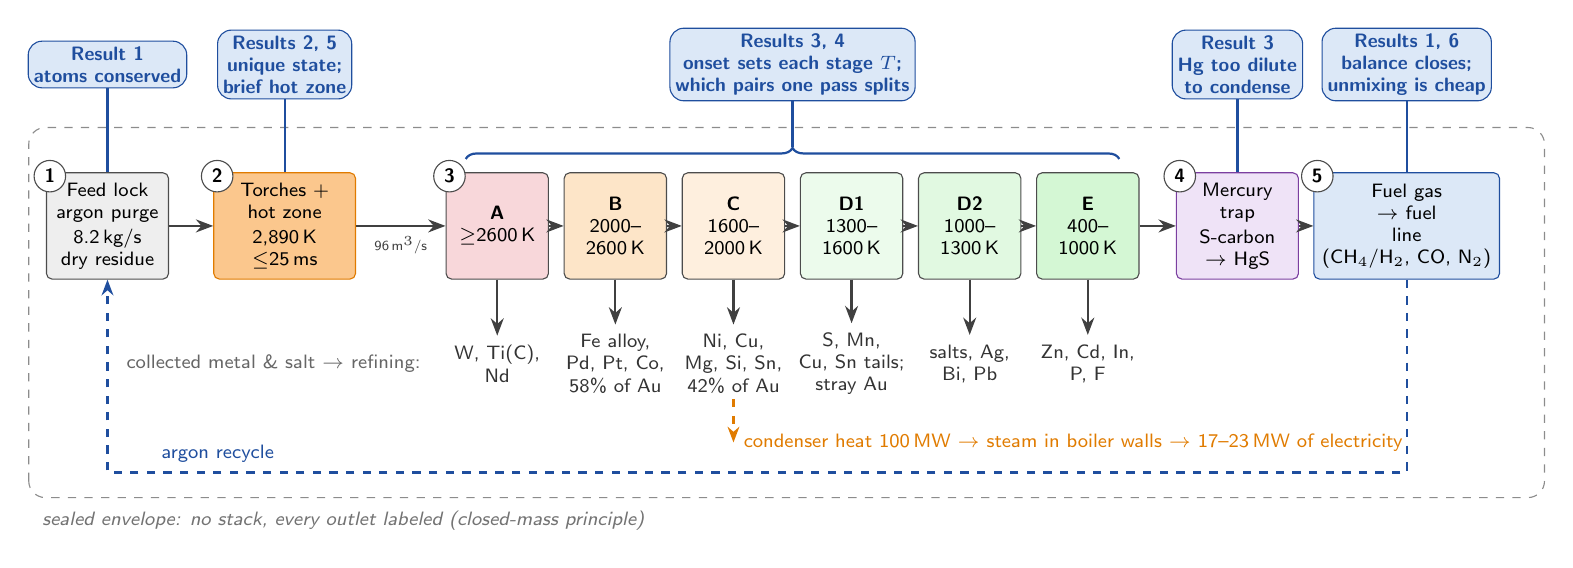
\begin{tikzpicture}[
  stn/.style={blk,minimum width=1.55cm,minimum height=1.35cm,font=\sffamily\scriptsize},
  cnd/.style={blk,minimum width=1.3cm,minimum height=1.35cm,font=\sffamily\scriptsize},
  prod/.style={font=\sffamily\scriptsize,align=center,text=black!80},
  res/.style={draw=dblue,fill=pblue,rounded corners=5pt,font=\sffamily\scriptsize\bfseries,
              text=dblue,inner sep=2pt,align=center},
  num/.style={circle,draw=black!70,fill=white,font=\sffamily\scriptsize\bfseries,inner sep=1pt,minimum size=4mm}]
% sealed envelope
\draw[dashed,black!45,rounded corners=6pt] (-1.0,-3.45) rectangle (18.25,1.25);
\node[font=\sffamily\scriptsize\itshape,text=black!55,anchor=north west] at (-0.95,-3.5)
  {sealed envelope: no stack, every outlet labeled (closed-mass principle)};
% stations
\node[stn,fill=pgrey] (feed) at (0,0) {Feed lock\\argon purge\\[1pt]8.2\,kg/s\\dry residue};
\node[stn,fill=porange,draw=dorange,minimum width=1.8cm] (hot) at (2.25,0)
  {Torches +\\hot zone\\[1pt]2,890\,K\\$\le$25\,ms};
\node[cnd,fill=ppink]   (A) at (4.95,0)  {\textbf{A}\\$\ge$2600\,K};
\node[cnd,fill=ppeach]  (B) at (6.45,0)  {\textbf{B}\\2000--\\2600\,K};
\node[cnd,fill=ppeach!60] (C) at (7.95,0)  {\textbf{C}\\1600--\\2000\,K};
\node[cnd,fill=pgreen!45] (D1) at (9.45,0)  {\textbf{D1}\\1300--\\1600\,K};
\node[cnd,fill=pgreen!70] (D2) at (10.95,0)  {\textbf{D2}\\1000--\\1300\,K};
\node[cnd,fill=pgreen]  (E) at (12.45,0) {\textbf{E}\\400--\\1000\,K};
\node[stn,fill=ppurple,draw=dpurple] (hg) at (14.35,0) {Mercury\\trap\\[1pt]S-carbon\\$\to$ HgS};
\node[stn,fill=pblue,draw=dblue] (cyl) at (16.5,0) {Fuel gas\\$\to$ fuel\\line\\(CH$_4$/H$_2$, CO, N$_2$)};
% flow
\draw[arr] (feed) -- (hot);
\draw[arr] (hot) -- node[below,font=\sffamily\tiny]{96\,m$^3$/s} (A);
\foreach \a/\b in {A/B,B/C,C/D1,D1/D2,D2/E,E/hg,hg/cyl} \draw[arr] (\a) -- (\b);
% products
\node[prod] (pA) at (4.95,-1.75) {W, Ti(C),\\Nd};
\node[prod] (pB) at (6.45,-1.75) {Fe alloy,\\Pd, Pt, Co,\\58\% of Au};
\node[prod] (pC) at (7.95,-1.75) {Ni, Cu,\\Mg, Si, Sn,\\42\% of Au};
\node[prod] (pD1) at (9.45,-1.75) {S, Mn,\\Cu, Sn tails;\\stray Au};
\node[prod] (pD2) at (10.95,-1.75) {salts, Ag,\\Bi, Pb};
\node[prod] (pE) at (12.45,-1.75) {Zn, Cd, In,\\P, F};
\foreach \s in {A,B,C,D1,D2,E} \draw[arr] (\s) -- (p\s);
\node[font=\sffamily\scriptsize,text=black!60,anchor=east] at (4.1,-1.75) {collected metal \& salt $\to$ refining:};
% station numbers
\foreach \s/\n in {feed/1,hot/2,A/3,hg/4,cyl/5} \node[num] at ($(\s.north west)+(0.05,-0.05)$) {\n};
% governing results
\node[res] (r1) at (0,2.05) {Result 1\\atoms conserved};
\node[res] (r25) at (2.25,2.05) {Results 2, 5\\unique state;\\brief hot zone};
\node[res] (r34) at (8.7,2.05) {Results 3, 4\\onset sets each stage $T$;\\which pairs one pass splits};
\node[res] (r3b) at (14.35,2.05) {Result 3\\Hg too dilute\\to condense};
\node[res] (r16) at (16.5,2.05) {Results 1, 6\\balance closes;\\unmixing is cheap};
\draw[dblue,thick] (r1) -- (feed);
\draw[dblue,thick] (r25) -- (hot);
\draw[dblue,thick,decorate,decoration={brace,amplitude=4pt,mirror}] (12.85,0.85) -- (4.55,0.85);
\draw[dblue,thick] (r34) -- (8.7,1.0);
\draw[dblue,thick] (r3b) -- (hg);
\draw[dblue,thick] (r16) -- (cyl);
% heat recovery and argon loop
\draw[darr,dorange] (7.95,-2.2) -- (7.95,-2.75) node[right,font=\sffamily\scriptsize,text=dorange]
  {condenser heat 100\,MW $\to$ steam in boiler walls $\to$ 17--23\,MW of electricity};
\draw[darr,dblue] (cyl.south) -- ++(0,-2.45) -| (feed.south);
\node[font=\sffamily\scriptsize,text=dblue,above] at (1.4,-3.12) {argon recycle};
\end{tikzpicture}
\end{document}
